\documentclass{article}

\usepackage[utf8]{inputenc}
\usepackage{url}
\usepackage{amsmath}
\usepackage{graphicx}
\usepackage{geometry}

\geometry{
a4paper,
left=30mm,
right=20mm,
top=30mm,
bottom=20mm,
}

\begin{document}

	\pagenumbering{gobble}
	\begin{center}

		{\LARGE Universidade Federal de Santa Catarina \par}
		\vspace {2cm}
		
		Ciências da Computação
		\vspace{2cm}

		Luca Fachini Campelli
		\vspace {4cm}

		\textbf{DESENVOLVIMENTO DE UM APLICAÇÃO PARA COLETA DE DADOS \\
				E EMISSÃO DE PASSAPORTES ELETRÔNICOS NA PLATAFORMA JAVACARD}
		\vspace {10cm}
		
		Florianópolis/SC \\

		2018
	\end{center}

	\newpage
	\begin{center}
		Luca Fachini Campelli
		\vspace{2cm}
		
		\textbf{\large DESENVOLVIMENTO DE UM APLICAÇÃO PARA COLETA DE DADOS \\
				E EMISSÃO DE PASSAPORTES ELETRÔNICOS NA PLATAFORMA JAVACARD}
		\vspace{2cm}

		\hfill \textbf{Trabalho de Conclusão de Curso \\}
		\hfill \textbf{para a graduação no curso de\\}
		\hfill \textbf{Ciências \hspace{18pt} da \hspace{18pt} Computação \\}
		\hfill \textbf{UFSC  \hspace{60pt}}

		\vspace{1cm}

		\hfill Florianópolis, 2018

	\end{center}

	\newpage

	\paragraph{\large Resumo}
		\begin{flushleft}
			\begin{large}
			\hspace{2cm} Com a preocupação com a segurança em todas as áreas, a identificação correta e segura das credenciais de uma pessoa se torna de extrema importância. A necessidade de vários documentos diferentes para as mais variadas funções faz surgir vários problemas, desde falsificação e roubo, até simples desorganização e perda.
O maior exemplo da necessidade dos mais variados documentos é em viagens internacionais. Nelas são necessárias diversas etapas até que se confirme a identidade do viajante afim de evitar falsificações, e outros tipos de ameaça, sendo o mais importante dos documentos o passaporte.\\
O intuito deste trabalho é criar uma infra-estrutura para emissão de passaportes eletrônicos na plataforma Javacard, baseado no padrão ICAO 9303 \cite{ICAO}, tendo em mente a segurança das informações. O sistema de emissão deverá prover um aplicativo que colete as informações do usuário, e crie um cartão dentro de uma das 5 possibilidades existentes e descritas no trabalho de conclusão de curso \cite{SASSO}.
Este cartão deve possuir todas as informações de identificação da pessoa, sendo desnecessário outro documento de identificação promovendo a idéia de cadastro único. 
O projeto será efetuado juntamente com o LabSec e o professor responsável, com a utilização da biblioteca JMRTD \cite{JMRTD}, que será adaptada para os fins deste projeto, e projetos anteriores do LabSec que servirão de base para desenvolvimento do produto final. 
	\vspace{1cm}

Palavras-chave: Javacard, Passaporte,JMRTD, Segurança, Identidade, Digital, Cadastro Unico
			\end{large}
		\end{flushleft}


	\paragraph{\large Abstract}
		\begin{flushleft}

			Dat stuff up thea

		\end{flushleft}
	
	\newpage

	\tableofcontents
	\newpage

	\pagenumbering{arabic}

	
	\section{Introdução}
		\begin{flushleft}
			\begin{large}
			\hspace{2cm}Com o aumento do compartilhamento de dados entre instituições de um mesmo grupo, a necessidade de segurança aumenta conforme o tamanho do grupo aumenta e a necessidade de confirmar a identidade de um usuário, para que não haja abuso dos recursos nem acesso irrestito aos dados se torna cada vez mais importante. Assim, cada vez mais cresce a quantidade de documentos necessários para que se confirme a identidade do usuário, como CPF, RG, CNH, Passaporte, e biometrias digitais que todos ficam armazenados em documentos físicos e separados, aumentando a quantidade de itens que uma pessoa tem que carregar, e aumentando o tempo para resgatar estas informações e conferir com o usuário. \\
			\hspace{2cm} Este trabalho visa o desenvolvimento de um sistema que controle a emissão de passaportes universitários eletrônicos baseado no padrão ICAO 9303, na plataforma Javacard \cite{JAVACHEN}. Este sistema deverá englobar todas as necessidade documentais para a identificação correta e segura do usuário, para agilizar processos de identificação biométrica. Ele deve coletar os dados do usuário como digitais, assinatura digitalizada, nome, e dados de identidade para a criação de um cartão Javacard eletrônico seguro, dentro dos vários modelos possíveis. Para tal serão utilizadas técnicas de criptografia para assegurar uma comunicação segura com o cartão, e seu funcionamento adequado. À seguir, serão discutidos alguns tópicos necessários ao entendimento destes conceitos.

			\end{large}
		\end{flushleft}

	\section{O que é segurança computacional? [\cite{STALLINS} - cap 1]}
		\begin{flushleft}
			\begin{large}
			\hspace{2cm} Segurança computacional engloba todas as áres de pesquisa relacionadas a manter algum tipo de informação segura, seja ela uma senha, listas de cadastros, um banco de dados, documentos ou uma receita de bolo. As pesquisas relacionadas a segurança computacional, trabalham para proteger estas informaçôes de pessoas que as poderiam utilizar para maus fins, seja impedindo que elas sejam obtidas ou entendidas por outras pessoas, ou garantindo que uma informação não foi alterada antes de ser entregue ao destinatário. As próximas seções deste documento explicam certos campos desta área que serão necessários ao entendimento do leitor:
			\end{large}
		\end{flushleft}

	\section{Criptografia Simétrica e Assimétrica [\cite{STALLINS} -parte 1 - parte 2]}
		\begin{flushleft}
			\begin{large}

 			\hspace{2cm} É possível cifrar a informação para que apenas quem possua a chave da cifra possa acessa-la. O ato de embaralhar o significado da mensagem se chama cifrar, e o inverso, decifrar. Para tal, utiliza-se algum tipo de algoritmo que, em conjunto com uma chave, seja capaz de mascarar a informação original e que seja reversível, para que com o uso da chave, se possa desfazer a criptografia e acessar o conteúdo original da mensagem. Nesta área existem dois tipos de protocolos para cifrar mensagens: a criptografia Simétrica e a Assimétrica. \\
			\hspace{2cm}Na criptografia simétrica, uma única chave é utilizada por ambas as partes, para cifrar e decifrar a mensagem. Neste contexto, as duas partes devem antecipadamente acordar a chave para ser usada entre sua comunicação. Na criptografia assimétrica, são utilizadas o que se chamam de chaves públicas e privadas. A chave pública é utilizada para cifrar, e apenas com a chave privada é possível se decifrar o conteúdo da mensagem, e vice-versa. Como o nome já diz, a chave privada é secreta, e pertence apenas a uma das partes entre as mensagens, já a chave pública é compartilhada pela rede e todos que tiverem interesse terão acesso à ela, assim, qualquer um pode enviar uma mensagem cifrada a um usuário, cifrando-a com a chave privada, e apenas o destinatário poderá lê-la. Devido às dificuldades de se utilizar este protocolo ele é mais utilizado para certiicações digitais.
			\end{large}		
		\end{flushleft}

	\section{Função Hash - SHA [\cite{STALLINS} - cap 11 - pg313]}
		\begin{flushleft}
			\begin{large}

    		\hspace{2cm} Esta função é amplamente utilizada para garantia de consistência tanto em criptografia quanto em várias outras áreas. Esta função funciona embaralhando os bits de uma mensagem à um ponto que seja impossível inverter o processo. Ela aceita uma mensagem de qualquer tamanho, porém sempre retornará uma cadeia de bytes de tamanho fixo, não importando qual seja a entrada. Porém a maior característica desta função está no fato de que para duas entradas diferentes x e y, sendo H(x) e H(y) o resultado depois de terem sido aplicados x e y respectivamente na função, nunca se deve encontrar um par tal que H(x) = H(y). Desta forma, é possível se checar a integridade de uma mensagem, aplicando a função hash sobre ela antes de ser enviada, e depois de recebida, e comparando as saídas, pois se a mensagem foi alterada, por menor que seja a alteração, os dois resultados da função serão completamente diferentes. O algoritmo mais utilizado para esta função é o SHA 2 - Secure Hash Algorithm 2(Algoritmo de Hash Seguro 2), projetado pela NSA, e possui seis versões diferentes, onde a mudança principal está no número de bits que eles retornam: SHA-224, SHA-256, SHA-384, SHA-512, SHA-512/224, SHA-512/256. 
			\end{large}
		\end{flushleft}

	\section{Assinaturas Digitais[\cite{STALLINS} - cap 13.1 - pg 395]}
		\begin{flushleft}
			\begin{large}

			\hspace{2cm}A confiança entre duas partes de uma troca de mensagens pode não ser suficiente para que informação sensível seja transferida. Uma parte “A” pode forjar uma mensagem alegando ter sido enviada pela parte “B”, ou “B” pode simplesmente negar ter enviado qualquer mensagem, mesmo que o tenha. Desta forma, um meio de proteger âmbas as partes contra fraude mútua são as assinaturas digitais.
    Uma assinatura digital consiste em uma mensagem “M” e uma assinatura. Esta assinatura consiste de “M” passada pela função Hash explicada acima, cifrada com a chave privada do remetente e concatenada à “M”. Desta forma, para o destinatário verificar a assinatura de “M”, ele deve separar a hash cifrada de “M”, decifrá-la com a chave pública do remetente, e então comparar o resultado com “M” passado novamente pela função Hash. Se ambos os resultados forem iguais, isto provará que o remetente não poderá negar que enviou a mensagem, pois foi assinado com sua chave privada, e o destinatário não poderá forjar ou modificar a mensagem pois ele não possui a chave privada do remetente.
			
			\end{large}
		\end{flushleft}


	\begin{figure}[hb!]
		\centering
		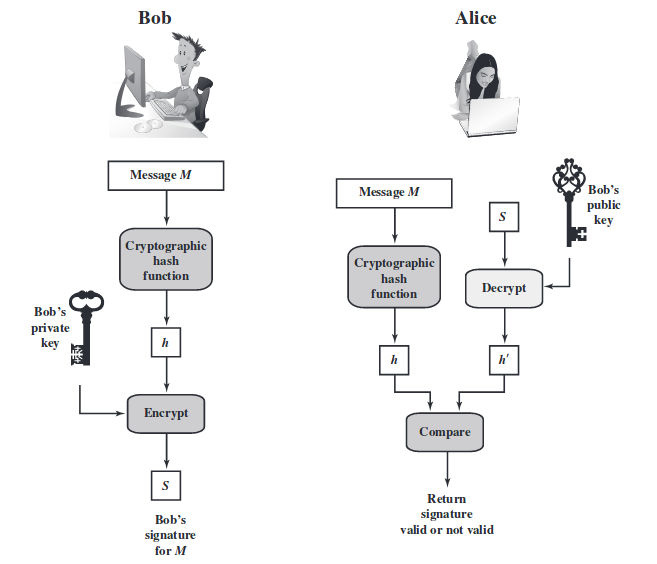
\includegraphics[width=250px]{AssinaturaDigital.png}
		\caption{Descrição simplificada do funcionamento de uma assinatura digital.}
		\label{fig:digiSign}

	\end{figure}

	\section{Certificados Digitais[\cite{STALLINS} - cap 14.4 - pg 435]}
		\begin{flushleft}
			\begin{large}
				
				\hspace{2cm}Certificados digitais são documentos eletrônicos que garantem a autenticidade de um certo elemento. Este que pode ser uma entidade, um site da internet ou um terminal de cartões. Um certificado é composto de algumas informações da entidade,  a chave pública da entidade, e uma assinatura digital sobre o certificado. Dependendo do tipo de certificado, esta assinatura adicionada ao final do documento é cifrada ou com a chave privada de quem o criou, denominado de certificado auto-assinado, ou com a chave privada de uma autoridade certificadora (CA - Certificate Authority). \\
				\hspace{2cm} Para que um certificado possua credibilidade, ele deve ser assinado por uma CA, e guardado em um servidor desta para que seja acessível. Para verificar a autenticidade de um certificado, deve-se separar o certificado C da hash H, decifrar a hash utilizando a chave pública da CA H’, e passar o certificado pela mesma função de hash utilizada em sua criação C’(que está incluído junto com as outras informações dentro do certificado). Se C’ for igual a H’ então pode-se confirmar que: Este certificado foi assinado pela CA e que nenhuma alteração foi feita à ele, pois como a função hash não possui duas respostas iguais para entradas diferentes, se o certificado for alterado, passando o certificado pela mesma função acarretará em uma hash diferente da que está ao final do documento, e, como ninguém mais possui a chave privada da CA, se a chave pública da CA decifrou com sucesso a hash, significa que quem a cifrou foi mesmo a CA, garantindo assim a credibilidade do certificado.

			\end{large}
		\end{flushleft}

    
	\section{Javacard\cite{JAVACHEN}}
		\begin{flushleft}
			\begin{large}

				\hspace{2cm} O Javacard é um cartão eletrônico que possui dois componentes principais, Um chip de contato e um processador interno. Este chip de contato se faz presente do lado externo do cartão, da mesma forma que cartões de crédito ou débito modernos, e cuida da comunicação do cartão com a leitora. O processador interno funciona como um computador, ele roda um sistema operacional Java, o que torna este cartão um Javacard. Ele também possui uma memória interna capaz de armazenar dados. Este sistema operacional pode possuir aplicativos em sua memória, e dependendo do programa que os acessar, pode escolher qual deles executar. O Chip de contato fornece energia e faz a comunicação entre a leitora ou terminal e o processador.

			\end{large}
		\end{flushleft}

    
	\section{O Documento ICAO 9303[1]}
		\begin{flushleft}
			\begin{large}
				\hspace{2cm} O documento ICAO 9303 será utilizado como base e padrão para toda formatação do aplicativo de passaporte.. ICAO é uma sigla para “International Civil Aviation Organization”, que é uma agência especializada das Nações Unidas. Foi estabelecida em 1944 para gerenciar a admnistração e governância da Convenção de Aviação Civil Internacional (Convenção de Chicago). \\
    			\hspace{2cm} O documento é escrito em 12 partes, cada uma descreve um aspecto sobre como um Passaporte Eletrônico deve ser desenvolvido, a primeira parte dando uma introdução sobre o as características de um passaporte eletrônico, e definindo siglas e acrônimos para os documentos seguintes.\\
    			\hspace{2cm} A segunda parte da especificações sobre a segurança física do cartão, desde o design interno, quanto a produção, transporte e criação do cartão. 


			\end{large}
		\end{flushleft}

    


	\section{}
		\begin{flushleft}
			\begin{large}
			\end{large}
		\end{flushleft}

\begingroup
	\section{Referências}
		\renewcommand{\section}[2]{}
		\begin{large}
		\bibliography{TCC}
		\bibliographystyle{plain}
		\end{large}
\endgroup
\end{document}
